\section{Introduction}
\label{sec:intro}
%\KZ{Be careful not to use ``context'' for ``premise''. We stick to the
%terminology ``premise'' and ``choices'' throughout this paper.}
%\KZ{MCNLR is kind of tasks that is made up of
%a context and two or more choices, all in text form.
%Recently, research has noted that some advanced NLP models
%may not be truly solving this type of questions by understanding
%the underlying logical connections between the context and the choices,
%but instead resorting to local signals in the choices alone.
%Such speculations were largely fueled by a kind of
%experiments called ``end-only tests''. Although such tests
%can show that models have some ability to predict correct choices
%without given the context, it doesn't show what the model does
%if it were given the full questions with the context.
%In this work ...  }
%main point:
%1. identify short circuit, dataset have some hints, spurious feature. 
%1. pretrained models perform very well on many tasks but fail on ``stress tests'' especially 
%the cases requiring to know specific relations between context and candidates, like coreference. 
%Thus there is an assumption that model learns a lot only from candidates.
%2. previous work try to explain this by candidate-only test, but it can't really judge if the model really 
%learn from candidates.We design another test called cross test...
%3. In this paper, we further study how to improve models by some simple data augmentation methods 
%based on the weakness of models. We target to teach models to look at both context and candidates. 

%Multiple-choice questions (MCQs) are a widely used format  
%in natural language understanding tasks. 

Large-scale neural networks have been applied extensively
to natural language reasoning (NLR) tasks such as
causal reasoning~\cite{copa2012}, 
story ending prediction~\cite{roc2017},
argument reasoning comprehension~\cite{arct2018}, and 
reading comprehension~\cite{yu2020reclor}.
Many of the current benchmarks of these NLR tasks take the 
form of multiple-choice questions (MCQs) which are made up 
of a premise and two or more choices. Below is an example taken 
from COPA~\cite{copa2012}, which tests commonsense causal 
reasoning.

\begin{example}\label{ex:copa}
An MCQ from COPA:\\ \\
\noindent
\textbf{Premise:} The man hurt his back.\\
\textbf{Choice 1:} He stayed in bed for several days.  \checksymbol \\
\textbf{Choice 2:} He went to see a psychiatrist. \crosssymbol 
\end{example}

Usually, models are trained on the training data and tested with the standard 
validation-test split paradigm.  While accuracy on held-out data is a useful
indicator, held-out datasets are often not diverse enough
and may contain the same biases in the training
data~\cite{mccoy2019right}. Furthermore, as simple aggregated statistics, 
accuracy on the test set doesn't show the robustness of the model,
or why a question is answered correctly. 
There has been speculation~\cite{endingonly1,zellers2018swag} that many models 
did not really ``understand'' the semantical and logical connection between
the premise and the choices, 
but do well only due to spurious statistical features in the choices, 
which means the models are actually fragile.

Such fragility can be observed by 
%Lately, some research has been devoted to 
%analysis the MCQs models by
both white-box and 
black-box tests.
%Inspired by previous work that uses the attention map to explain the 
%performance of neural models on such natural language~(NL) reasoning problems,
In a white-box test~\cite{vig-2019-multiscale}, attention map between the words in the full question 
from the final encoder layer of the model can reveal the
connection, or the lack of one, between the premise and the choices. 
\figref{fig:att-goodex}, which is a plot for \exref{ex:copa},
clearly shows that there's virtually no connection between the first choice
and the premise (highlighted by the red box) when BERT is processing
the full question. While the attention between the words within the
first choice remains the same when the model processes only the choices
without the premise. 
%\KZ{This fig doesn't seem to show choice-only situation?} 
We call such a phenomenon ``short circuit'' in multiple-choice 
NLR in this paper. 
%And we also use ``choice only'' test as a kind of indicator 
%for ``short circuit'' in our experiment.

\begin{figure}[th!]
\centering
\includegraphics[width=0.6\columnwidth]{figure/end_related.eps}
\caption{Attention map showing that BERT short-circuits on a COPA question.}
\label{fig:att-goodex}
\end{figure}

%Due to the limited interpretability of deep neural models, 
Furthermore, two kinds of black-box tests have been attempted.
One is called ``ending-only tests'' in some literature~\cite{endingonly1,endingonly2}, 
which we refer to as ``choice-only test'' here since 
our focus is on MCQs.
For example, BERT, when fine-tuned on the COPA data, can answer
the question in \exref{ex:copa} correctly. When we remove the premise from 
the same question and feed it to the model, it still
gets the correct answer~(Choice 1). This result from the ``choice-only'' 
test seems to suggest that the model can make correct predictions
without even looking at the premise. 
The other blackbox test is a kind of stress test~\cite{checklist2020acl}, 
which tests if the model is short-circuiting toward (or against) certain linguistic features
such as named entities, typos, and negations.
%It breaks down potential capability failures into specific behaviors. 
In this work, we apply many stress test cases of several categories, 
and observe that many models are fragile with low accuracies.
Through the above tests, we are able to confirm that three popular 
deep models, i.e., BERT, XLNet~\cite{xlnet2019nips} and 
RoBERTa~\cite{roberta2019}, when applied to multiple-choice NLR, 
all suffer from the ``short-circuit'' problem.

%We call the phenomenon ``\textit{short circuit}'' in natural language 
%reasoning in this paper. 

%Despite the previous research advocating the choice-only test,
%we argue that it has an inherent flaw as a test for
%short circuit: just because the model answers correctly without
%the premise doesn't mean the model doesn't look into the premise
%when it's given one. What we need is a test that works with questions
%that are complete with premises and choices.
%\begin{figure}[th]
%\centering
%\includegraphics[width=\columnwidth]{figure/end_unrelated.eps}
%\caption{BERT passes the choice-only test but 
%doesn't short-circuit on another COPA question (left).}
%\label{fig:att-badex}
%\end{figure}
%
%Can we achieve the same purpose using
%the choice-only test? The answer is negative. \figref{fig:att-badex}
%shows another question which is correctly answered by BERT with
%or without the context, but the attention map shows that 
%there exists some attentions between
%the word ``forgot'' in the choice and some other words in
%the context, indicating that the model is not really short-circuiting.

%we first develop an intuitive method to visualize
%the model's attention map to verify if it is shortcircuiting. 

%Manually checking the short circuit of a model using such attention maps
%is tedious and costly. And automating this process would require the access to 
%the code of the models and such approach only works for 
%attention-based models.

%To address these challenges, we design a new operation on 
One straightforward way to 
%improve the model robustness 
reduce the model short circuits is to train
the models with hard cases that look like the stress tests. 
However, many stress tests are constrained by the way choices
are constructed, which limits the quantity of cases to automatically generate, 
and consequently their ability to serve as general 
data augmentation methods. Besides, most of the stress tests are feature specific 
and hard to generalize.
%\KZ{Is quantity is the only reason to
%use crossover and mutation? This sounds a bit weak..}
To this end, we propose \textit{crossover} and 
\textit{mutation} operators, which can easily generate abundant data and 
encourage models to pay more attention to the premise. 
%MCQ question instances, 
%called \textit{crossover},
%which takes two MCQs and exchange their
%choices, analogous to how chromosomes swap their segments ino
%the biological reproduction. 
%Fortunately, crossover, as well as its counterpart operator \textit{mutation}, 
%do satisfy all the stringent requirements. 
%It imposes a unique challenge on models  
%frequently exploiting short circuit and is able to detect such behavior 
%on real tasks by constructing proxy test cases. 
%Through the lens of crossover test and  
%several other instance-level stress tests, such as named entity replacement, 
%we find evidence of short circuit and brittleness in three recent powerful natural language
%reasoning models reflected by notable declines in accuracy on these tests.
We apply crossover and mutation 
to augment the three models on ROC~\cite{roc2017}, COPA, 
ARCT~\cite{arct2018}, and RECLOR~\cite{yu2020reclor} and see 
up to 42\% increase in accuracy on the stress tests and 10\% increase in
the original test data, beating the previous strong baseline
back-translation~\cite{back2019}.
%\KZ{The following needs to be rewritten: 
%Through crossover test, we further confirm that many classifiers 
%based on pretrained language models do rely heavily on the 
%spurious features of the options on some test instances. 
%In addition, we follow previous work~\cite{} to generate several stress test for 
%model testing. Many models have experienced a significant 
%decline in the correctness of stress tests which also indicates 
%that models that learn short circuits are not robustness.
%}

%Different with previous research~\cite{} which create a more robust model 
%by changing the structure of the model to adversarial training. 
%For the above issue, we mainly investigate two simple data augmentation methods 
%with no changes to models in this paper: 
%\textit{cross data augmentation} and \textit{grammar data augmentation}. 
%Based on the model's excellent performance on various tasks, 
%we believe the pretrained models are capable of learning reasoning knowledge 
%but are affected by spurious features in dataset and perform poorly on stress test. 
%By augmenting more data with these two methods, the pretrained models can consider more 
%about contextual relationships rather than just making judgments through choices. 
%We explain and analyze the reasons for the model improvement by 
%increasing on stress test and visualizing the model's attention matrix. 


This paper makes the following contributions:
%\item We design ``crossover'' test as a blackbox proxy test to 
%massively and efficiently detect short-circuiting problem.  
%\item We propose a black-box proxy test framework for detecting short circuits, and 
%particularly ``crossover'' test which is shown to be effective in this framework.
i) we propose the crossover and mutation operations
to augment training data that teaches the models to pay attention to
the premises in questions; ii) experiments show that the augmented models 
perform substantially better on diverse stress tests while maintaining their
accuracies on the original tests, demonstrating reduced short circuits;
iii) we provide evidence to show that method indeed reduces 
short-circuits in these models, thus confirming the 
validity of our approach.

%\begin{figure*}[th]
%\centering
%\begin{subfigure}[b]{0.49\textwidth}
%\centering
%\includegraphics[width=\columnwidth]{figure/end_related.eps}
%\caption{Cue ``no'' in MNLI}
%\label{fig:cue_no}
%\end{subfigure}
%\hfill
%\begin{subfigure}[b]{0.49\textwidth}
%\centering
%\includegraphics[width=\columnwidth]{figure/end_unrelated.eps}
%\caption{}
%\label{fig:cue_threw}
%\end{subfigure}
%\caption{Three test examples for distribution comparison with 4 different models}
%\label{fig:cue_result}
%\end{figure*}





%questions to discuss:
%1. how to know if a model only pay attention to candidates only? ending only? cross? 
%2. how to know if a model have a poor performance on stress test?
%word swap  choice swap(premise) reflecility (aug merge)
%3. how to explain typo and synonym? should we use grammar to test? do we have other relational stress tests?
%we only have pronoun, negation, ner now. adverbial, synonym paraphrase right to right, typo
%4. experiment should try on different test cases many times or same cases many times?
